\section{Mouse embryonic fibroblasts reprogramming dataset}\label{apdx:mef}

We consider the mouse embryonic fibroblasts (MEF) reprogramming dataset of \cite{schiebinger2019optimal}. It consists of $p=19,089$ gene expressions for $251,203$ MEF cells, densely sampled across $18$ days, with $39$ individual timepoints. The experiment involves adding Doxorubicine (Dox) to the cells on day 0, withdrawing it at day 8, and then transferring them to either a serum-free N2B27 2i medium or maintaining them in serum. 

\paragraph*{Objective.} We would, therefore, want to produce a representation, using our Soft Mapper optimization, that accounts for the time component (like in Section~\ref{subsec:single-cell}) and for the divergence in the treatment that the cells received at day 8.
In order to achieve this, we first take a uniformly sampled subsample of the dataset of size $n=1,500$ and we use the same preprocessing procedure as with the human preimplantation dataset. Similarly, we consider the same settings (linear family of filter functions, smooth cover assignment scheme, agglomerative clustering, diagonal initial parameter set and extended total persistence), and we run Algorithm \ref{alg1} with $N=300$ and $M=10$.
The learning curve is displayed in Figure \ref{fig:ot_curve}. 

\begin{figure}[H]
    \centering
    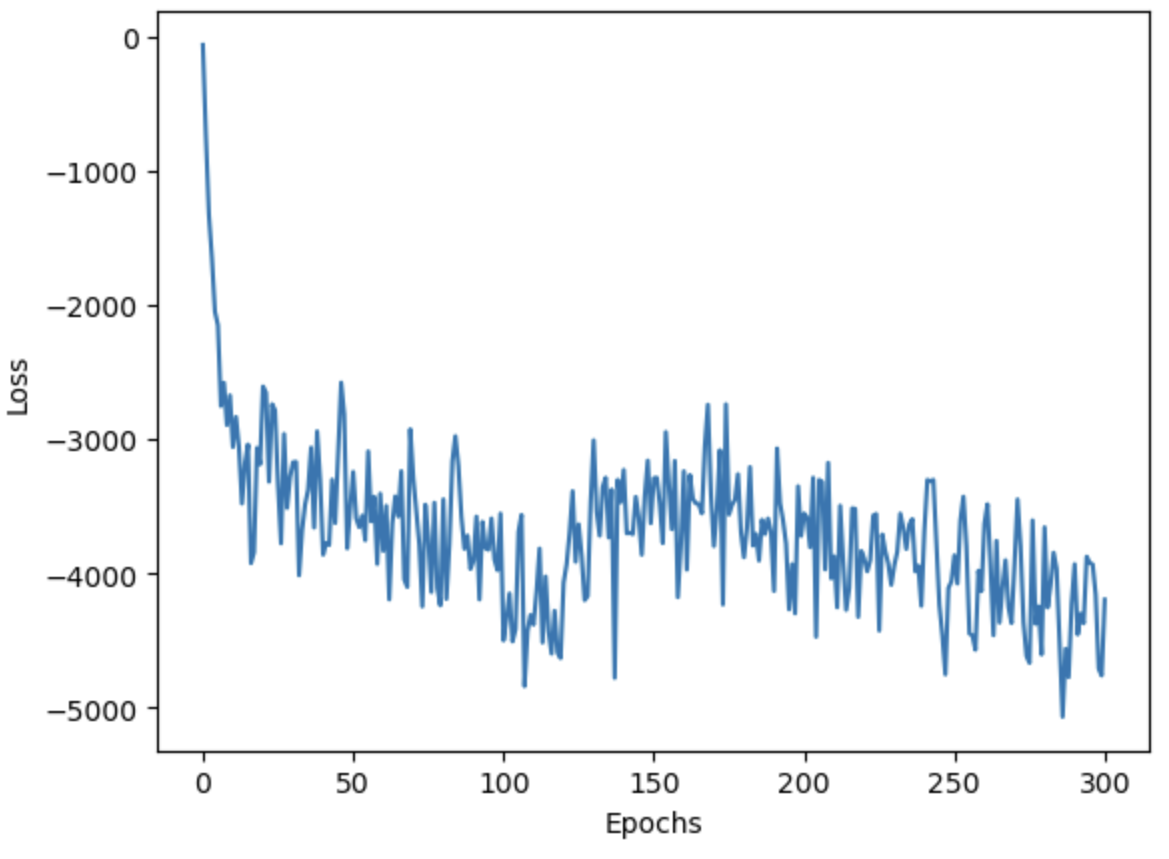
\includegraphics[width=.3\textwidth]{./ot_curve.png}
    \caption{Learning curve for the MEF reprogramming dataset.}
    \label{fig:ot_curve}
\end{figure}

\paragraph*{Qualitative assessment.} By looking at the standard Mapper graphs corresponding to the initial and the optimized filter functions in Figure \ref{fig:ot_mappers}, one can see that the optimized Mapper graph represents the time component better and that it shows two major branches, which point to the two phases that appear in day 8 of the experiment. These observations are confirmed by the improvement in the Pearson's correlation coefficients with respect to time between the initial and the optimized filter function values in Table \ref{tab:ot_pearsonr}. We also color the optimized Mapper graph in Figure \ref{fig:ot_phases} using the three phases in the experiment (Dox, 2i and Serum), each mapped to a different color channel.

\begin{figure}[H]
    \centering
    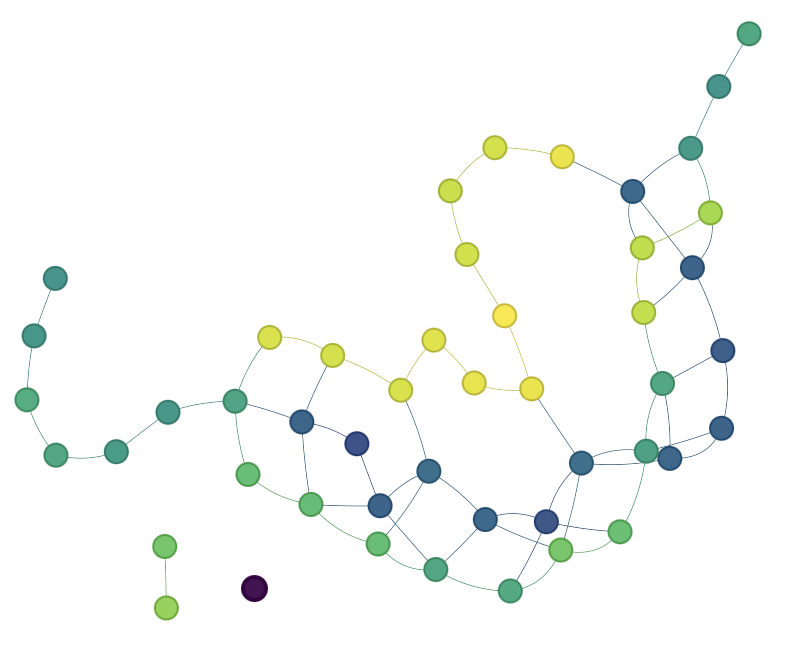
\includegraphics[width=.3\textwidth]{./ot_initial.png}\hfill
    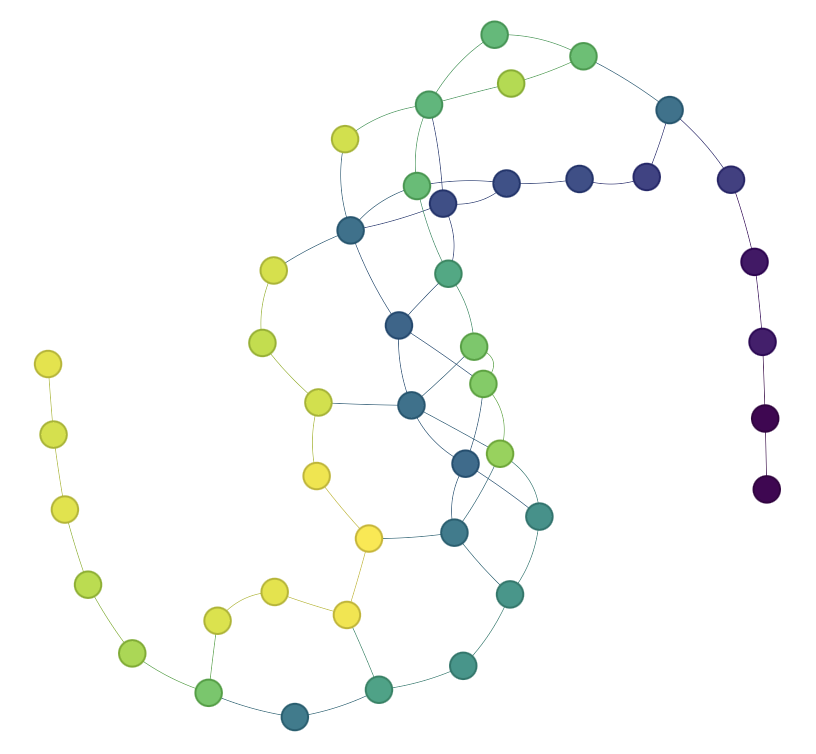
\includegraphics[width=.3\textwidth]{./ot_final.png}
    \caption{Classical Mapper graphs for the MEF reprogramming dataset computed using: in the left the initial filter function and in the right the optimized filter function. Vertices are colored using the mean value of the sampling timepoint in the corresponding clusters.}
    \label{fig:ot_mappers}
\end{figure}
\begin{table}[H]
    \centering
    \begin{tabular}{|c|c|c|}
    \hline
    Filter & Correlation with time & P-value\\
    \hline
     Initial    &  -0.0560 & 2.9882e-02\\
     \hline
     Optimized    & -0.4015 & 3.2090e-59\\
     \hline
    \end{tabular}
    \caption{Pearson's correlation between the initial filter and time, and the optimized filter and time. The associated $p$-values, obtained from testing the null hypothesis that the true correlation coefficient is zero, are also presented.}
    \label{tab:ot_pearsonr}
\end{table}
\begin{figure}[H]
    \centering
    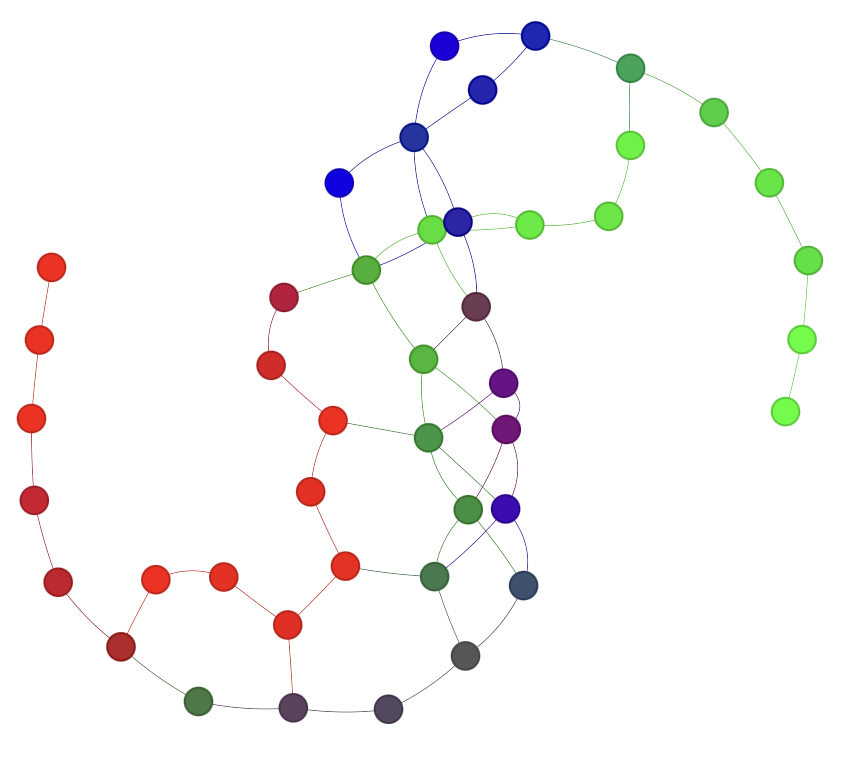
\includegraphics[width=.3\textwidth]{./ot_phases.png}
    \caption{Standard Mapper graph computed using the optimized filter function, colored by mapping each phase to a color channel: Dox in green, Serum in blue and 2i in red.}
    \label{fig:ot_phases}
\end{figure}
